\section{Experimental setup}
\label{sec:setup}
The MB events in p--Pb collisions at $\snn$~=~5.02~TeV used for the present analysis were recorded using the ALICE detector in 2016. The center-of-mass reference system in p--Pb collisions is shifted by $\Delta y_{\mathrm{cms}} =$~0.465 units of rapidity along the direction of the proton beam. In the following, the convention that $y$ stands for $y_{\mathrm{cms}}$ is used. The ALICE apparatus used during the LHC Run 2 is described in detail in Ref.~\cite{Abelev:2014ffa}. The present analysis is carried out using the following detectors: V0~\cite{ALICE:2013axi}, the Zero Degree Calorimeters (ZDC)~\cite{Cortese:2019nnv}, the Inner Tracking System (ITS)~\cite{ALICE:2010tia}, the Time Projection Chamber (TPC)~\cite{Alme:2010ke}, and the Time-Of-Flight (TOF)~\cite{Jacazio:2018slq}. 

The V0 detector is a hodoscope of scintillators, located on both sides relative to the interaction point (IP), consisting of V0A and V0C, each made of 32 plastic scintillator strips, covering the full azimuthal angle within the pseudorapidity intervals $2.8 < \eta < 5.1$ and $-3.7 < \eta < -1.7$, respectively. The MB events are selected with a signal given by a hit in both the V0A and V0C in p--Pb collisions. The V0A on the Pb-going side provides the multiplicity class using the sum of the V0A signals at the same time. The collected MB sample corresponds to an integrated luminosity of 0.3~nb$^{-1}$~\cite{ALICE:2014gvw}. The ZDC detects nucleons emitted from the colliding nucleus by nuclear de-excitation processes or knocked out from wounded nucleons, the so called “slow” nucleons. Two identical sets of the ZDC, each composed of a neutron (ZN) and a proton (ZP) calorimeters, are located at 112.5 m from the ALICE IP on both sides, covering very forward rapidity regions. The ZDC provides the least biased centrality selection in p--Pb collisions~\cite{ALICE:2014xsp}.

The primary vertex position is reconstructed using the measured track segments in the Silicon Pixel Detector (SPD)~\cite{Santoro2009:ALICESPD}, the innermost two layers of the ITS. The primary vertex along the beam direction ($z_\mathrm{vtx}$) is required to be in $|z_\mathrm{vtx}|<10$~cm from the nominal point ($z_\mathrm{vtx}=0$). The distance between the primary vertex and an additional vertex is requested to be larger than 0.8~cm to reduce the pileup. In addition, the inconsistency between the number of track candidates in the ITS and clusters in the SPD vetoes the pileup. The probability of pileup events is expected to be about 0.5\% in MB events. The TPC is the main tracking detector of ALICE. The TPC covers the pseudorapidity range $|\eta|<$~0.9 over the full azimuth in a uniform solenoidal magnetic field of 0.5~T along the beam axis. The TPC is able to reconstruct charged particles down to $p_{\rm{T}}=$~0.15~GeV/$c$. Particle identification (PID) can be performed with the TPC and TOF. The TPC measures ionization energy loss $\mathrm{d}E/\mathrm{d}x$ of charged tracks to separate particle species. The TOF helps PID by measuring the flight time of charged particles from the primary vertex to the TOF.

\section{Data analysis}

The \fzero~resonances are reconstructed via the decay channel of \fzero~$\rightarrow \pi^{+}\pi^{-}$, where the branching ratio is reported to be B.R. = $46\pm6$\%~\cite{Stone:2013eaa}. Each charged pion reconstructed in the TPC is required to have $p_{\rm{T}}>$~0.15~GeV/$c$ and $|\eta|<$~0.8 for a uniform detector acceptance. The reconstructed tracks are required to satisfy the standard selection criteria, as reported in~\cite{ALICE:2022qnb}, to guarantee that only tacks with high quality are selected. To ensure good track momentum resolution, the reconstructed tracks are required to have at least 70 reconstructed points (out of a maximum of 159) in the TPC and two hits in the ITS, with at least one in the SPD. Selection criteria dependent on $p_{\mathrm{T}}$ are applied to the distance of closest approach to the primary vertex in the transverse ($d_{z}$) and longitudinal ($d_{xy}$) directions, requiring $d_{z}<$~2~cm and $d_{xy}<$~(0.0105~$+$~0.0350~$\times p_{\mathrm{T}}^{-1.1})$~cm, respectively, to suppress contamination from secondary charged particles originating from weakly decaying hadrons and interactions with the material.

The identification of charged pions is performed using the combined information of the TPC and TOF. The difference between the measured ionization energy loss and the prediction of the Bethe-Bloch parameterization obtained assuming the particle is a pion is required to be within two standard deviations for the pion identification in the TPC. The difference between the measured time-of-flight of the particle and the time expected for a pion is required to be within three standard deviations for the particle to be identified as pion in the TOF. The TOF signal is not used for PID when it is not originated from the reconstructed track. In this case, the TPC is used for the identification as a standalone detector.

\label{sec:ana}
\begin{figure}[hbt!]
	\centering
	\subfigure{ 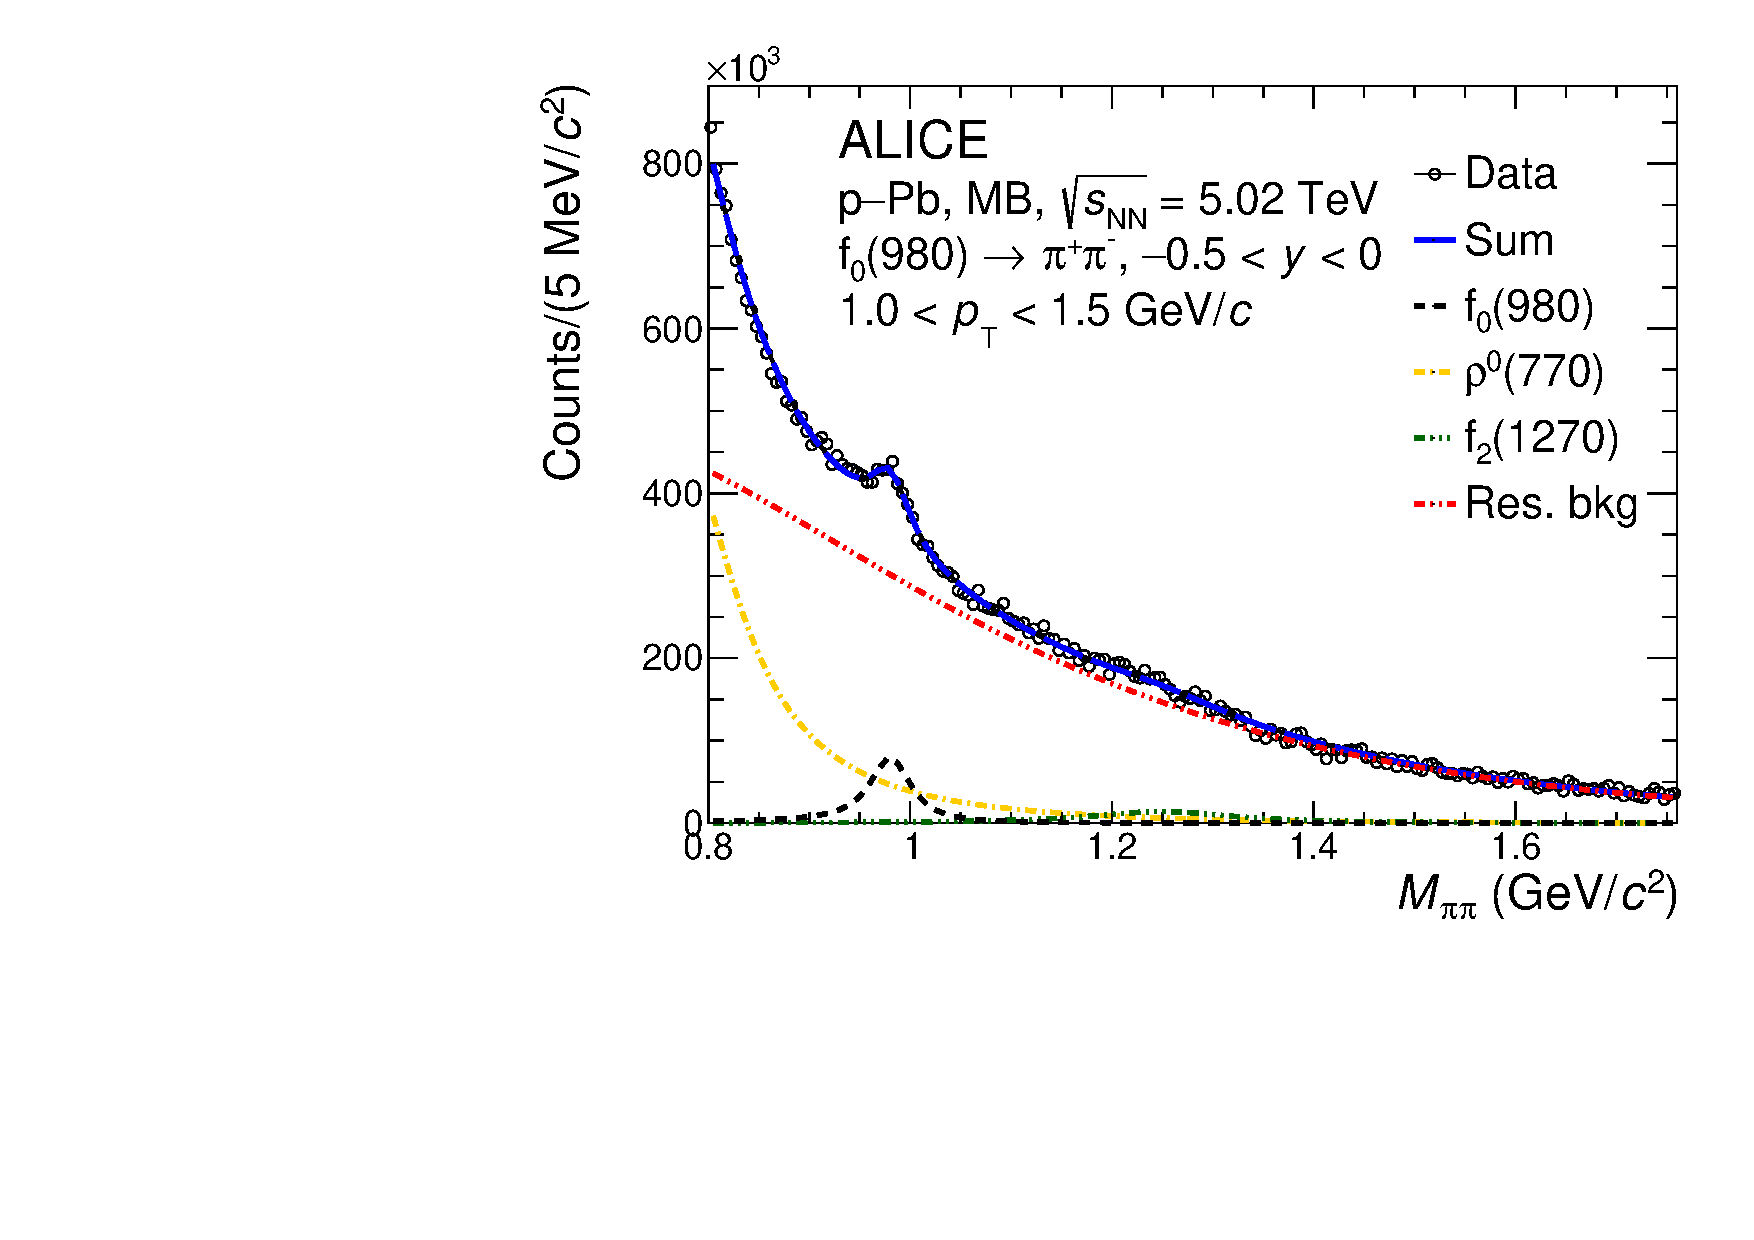
\includegraphics[width=0.47 \textwidth]{figures/Fig1_sigext_mb_pt0.pdf} }
	\subfigure{ 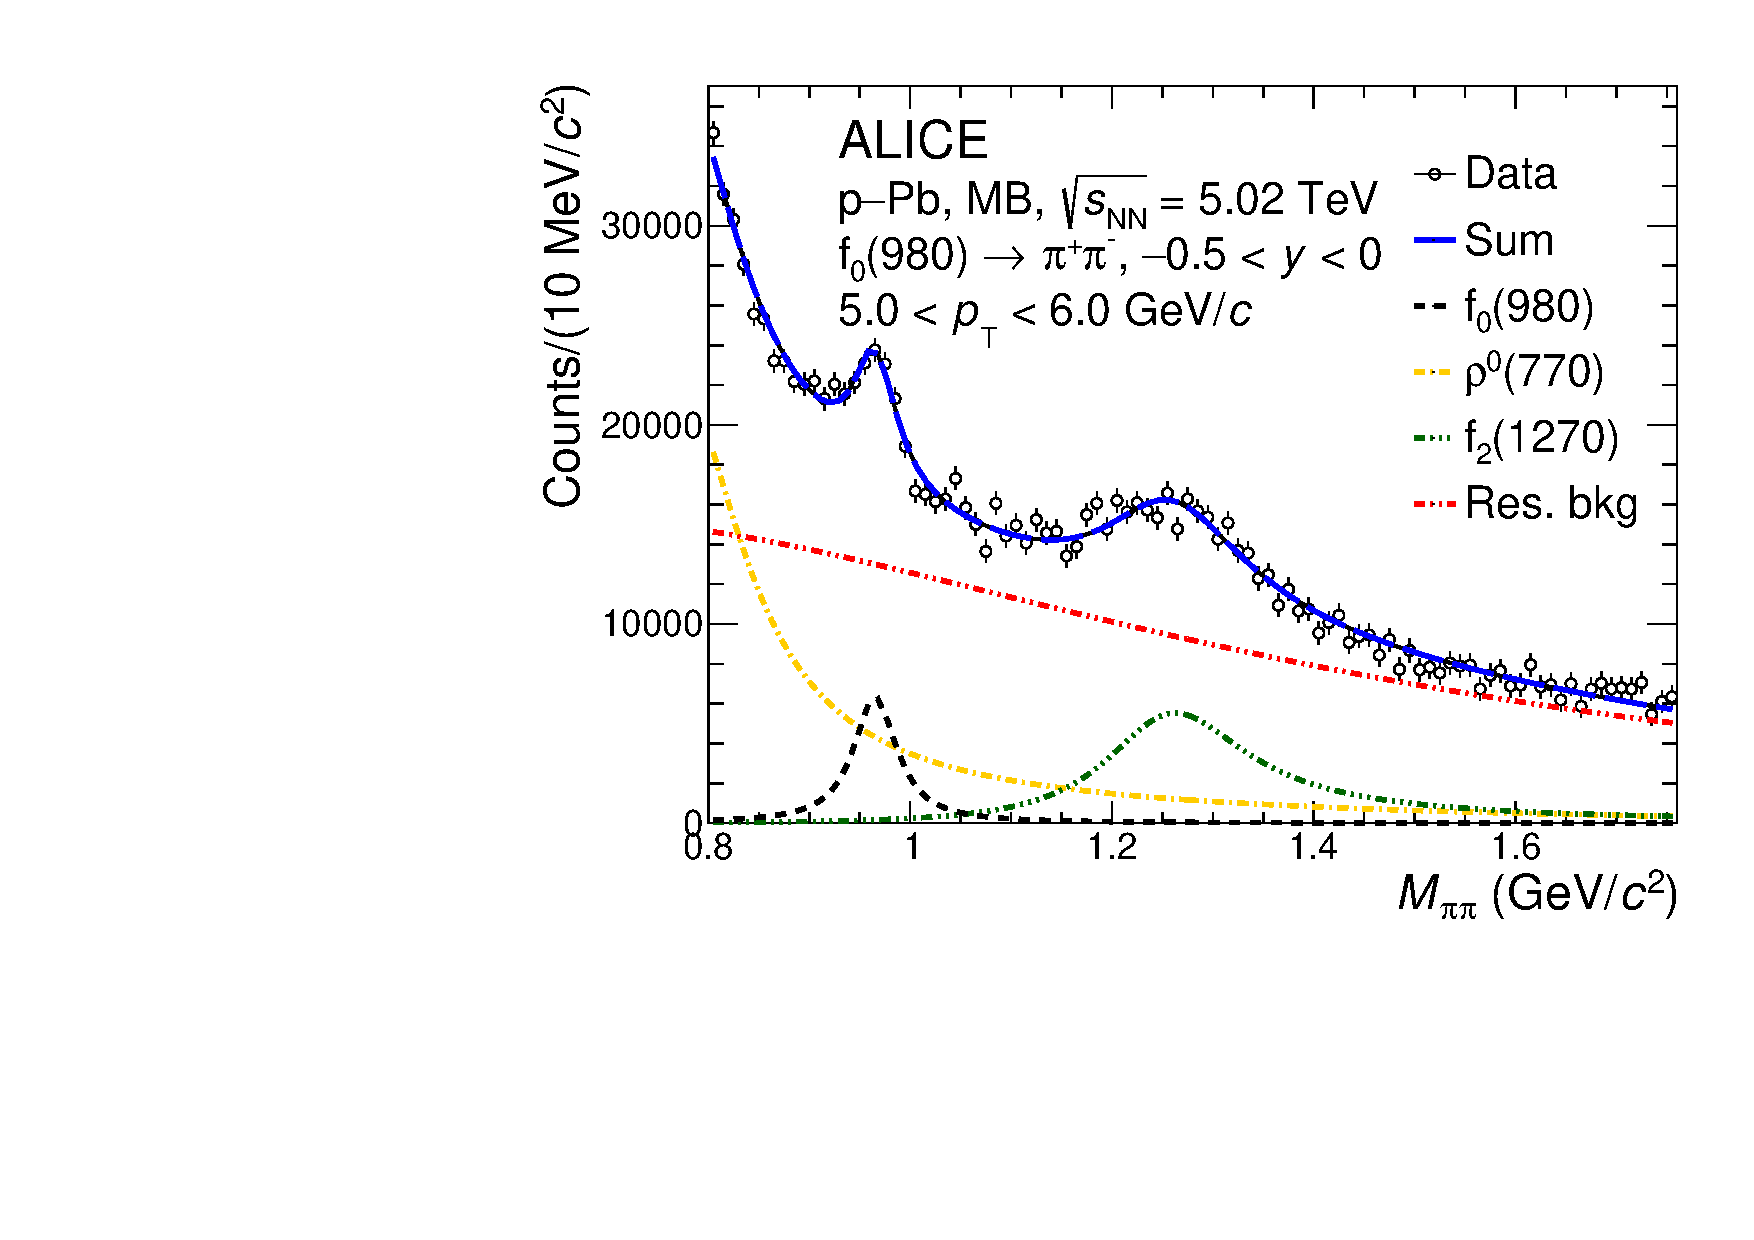
\includegraphics[width=0.47 \textwidth]{figures/Fig1_sigext_mb_pt1.pdf} }
	\caption{ Invariant mass distribution of $\pi^{+}\pi^{-}$ pairs in $-0.5<y<0$ after the like-sign background subtraction in p--Pb collisions at \snn~=~5.02~TeV. The left (right) plot is obtained at low (high) $p_{\mathrm{T}}$ of $\pi^{+}\pi^{-}$ pairs in non-single diffraction (NSD) events. }
	\label{fig:SigExt}
\end{figure}

The \fzero~signals are extracted using the invariant mass analysis by associating two opposite-charge pions in the same event at $-0.5<y<0$~\cite{ALICE:2013wgn}. The combinatorial backgrounds are subtracted using the like-sign method~\cite{LIKESIGN}. The like-sign background is constructed as the geometric average of $\pi^{+}\pi^{+}$ and $\pi^{-}\pi^{-}$ distributions,  2$\sqrt{N_{\pi^{+}\pi^{+}}N_{\pi^{-}\pi^{-}}}$. After subtracting the like-sign backgrounds from the $\pi^{+}\pi^{-}$ distribution, peaks of resonances decaying to $\pi^{+}\pi^{-}$ can be identified. Figure~\ref{fig:SigExt} shows the like-sign-subtracted $\pi^{+}\pi^{-}$ invariant mass distributions for 1.0~$<p_{\rm{T}}<$~1.5~GeV/$c$ (5.0~$<p_{\rm{T}}<$~6.0~GeV/$c$) in MB events on the left (right) panel. Because \rhoz~and $\rm{f}_{2}$(1270) dominantly decay to $\pi^{+}\pi^{-}$ and have large widths, \fzero~signals are overlapped with contributions from those two resonances. Residual backgrounds ($f_{\mathrm{bkg}}$) are mainly attributed to misidentified particles and mini-jets, which are represented as red-dashed-dotted lines in Fig.~\ref{fig:SigExt}. Each resonance contribution is described with a relativistic Breit-Wigner function (rBW)~\cite{ALICE:2018qdv, ALICE:2022qnb}. Note that detector resolution gives a negligible contribution to the estimate of the widths of broad resonances~\cite{ALICE:2016sak}. The rBW can be expressed as
\begin{eqnarray}
\mathrm{rBW}(M_{\pi\pi}) = \dfrac{AM_{\pi\pi}\Gamma(M_{\pi\pi})M_{0}}{(M_{\pi\pi}^{2}-M_{0}^{2})^{2} + M_{0}^{2}\Gamma^{2}(M_{\pi\pi})},
\label{eq:rBW}
\end{eqnarray}
where $\Gamma(M_{\pi\pi})$ is defined as
\begin{eqnarray}
\Gamma(M_{\pi\pi}) = \left[ \dfrac{ (M_{\pi\pi}^{2} - 4m_{\pi}^{2}) }{ (M_{0}^{2}-4m_{\pi}^{2}) } \right]^{(2J+1)/2} \times \dfrac{\Gamma_{0}M_{0}}{M_{\pi\pi}} .
\label{eq:rBWW}
\end{eqnarray}
Here, $A$ and $M_{0}$ are the amplitude of the rBW and the rest mass of the resonance, respectively. The rest width of the resonance, the spin, and the charged pion mass of 139.5~MeV/$c^{2}$ are represented as $\Gamma_{0}$, $J$, and $m_{\pi}$, respectively. The spins for \fzero, \rhoz, and $\mathrm{f}_{2}$(1270) are 0, 1, and 2, respectively. The $f_{\mathrm{bkg}}$ is fitted with a Maxwell-Boltzmann-like distribution, which can be expressed as~\cite{OPAL:1998enc}
\begin{eqnarray}
f_{\mathrm{bkg}}(M_{\pi\pi}) = B(M_{\pi\pi}-2m_{\pi})^{n}\exp{(c_{1}M_{\pi\pi} + c_{2}M_{\pi\pi}^{2})},
\label{eq:bkg}
\end{eqnarray} 
where, $B$, $n$, $c_{1}$, and $c_{2}$ are free parameters. Each rBW of the resonance is corrected for the $\pi\pi$ interference~\cite{ALICE:2018qdv, Rapp:2003ar}, which can be expressed as
\begin{eqnarray}
\mathrm{PS}(M_{\pi\pi}) = \dfrac{M_{\pi\pi}}{\sqrt{M_{\pi\pi}^{2}+p_{\mathrm{T}}^{2}}}\times\exp{(-\sqrt{M_{\pi\pi}^{2}+p_{\mathrm{T}}^{2}}/T_{\mathrm{kin}})},
\label{eq:ps}
\end{eqnarray} 
where $p_{\mathrm{T}}$ in the above equation denotes the transverse momentum of the $\pi\pi$ pair, and $T_{\mathrm{kin}}$ is the kinetic freeze-out temperature, set to be 160~MeV~\cite{ALICE:2018qdv} for all the defined multiplicity classes

The signal extraction carefully considers the width of the \fzero~as the width is not yet constrained by measurements (10~$<\Gamma_{0}^{\mathrm{f}_{0}}<$~100~MeV/$c^{2}$~\cite{ParticleDataGroup:2022pth}). The total fit function consists of the sum of three rBWs, one for each resonance and one function for the background, $f_{\mathrm{bkg}}$. This function has nine free parameters: 3 for \fzero~resonance (mass, width, and amplitude), two amplitudes for \rhoz~and f$_{2}$(1270) resonances, and 4 for $f_{\mathrm{bkg}}$. The masses and widths of \rhoz~and $\mathrm{f}_{2}$(1270) are well defined in Ref.~\cite{ParticleDataGroup:2022pth}, and those are fixed to $m_{\rho}=$~775.3~MeV/$c^{2}$, $\Gamma^{\rho}_{0}=$~~149.1~MeV/$c^{2}$, $m_{\mathrm{f}_{2}}=$~1,275.5~MeV/$c^{2}$, and $\Gamma^{\mathrm{f}_{2}}_{0}=$~186.7~MeV/$c^{2}$ during all fit procedures. Due to the many free parameters in the fit function, the procedure is split into three steps to prevent parameter values from converging in local minima. The purpose of the first step is to obtain an unbiased and initial \fzero~width. This step is performed using the MB sample over a wider $p_{\mathrm{T}}$ range to reduce the effect due to the statistical fluctuations. All nine parameters are left free. The second step aims at constraining the $f_{\mathrm{bkg}}$. The \fzero~width is fixed with the value determined in the previous step. The last fit procedure is processed with the fixed $f_{\mathrm{bkg}}$, while the \fzero~width is allowed to vary in the range of 10~$<\Gamma_{0}^{\mathrm{f}_{0}}<$~100~MeV/$c^{2}$. In each step, the amplitudes of three resonances and the mass of the \fzero~are left free, and the fit range is set to 0.8~$<M_{\pi\pi}<$~1.76~GeV/$c^{2}$.


While for the \fzero~analysis performed in pp collisions~\cite{ALICE:2022qnb}, the width is constrained to be 55 MeV/$c^{2}$, the present analysis leaves the \fzero~width as a free parameter. In the previous analysis, no phase space correction was applied. On the other hand, the present analysis considers the phase space correction for a possibly larger probability of $\pi\pi$ interference~\cite{STAR:2003vqj} owing to higher multiplicity in p--Pb collisions. It is found that consistent invariant yields are obtained from the two different analysis methods.

Raw yields of \fzero~($N_{\mathrm{f}_{0}}$) are obtained by integrating the \fzero~rBW function in the measured $p_{\mathrm{T}}$ range and corrected for the acceptance, the tracking efficiency, and the PID efficiency and then normalized for the event selections and the B.R.~\cite{Stone:2013eaa}. The fully corrected yield can be expressed as
\begin{eqnarray}
\dfrac{1}{N_{\mathrm{NSD}}}\dfrac{\mathrm{d}^{2}N}{\mathrm{dyd}p_{\mathrm{T}}} = \dfrac{1}{N_{\mathrm{evt}}} \dfrac{ N_{\mathrm{f}_{0}} }{ \Delta y \Delta p_{\mathrm{T}} } \dfrac{  \epsilon_{\mathrm{trig}} f_{\mathrm{vtx}} f_{\mathrm{SL}} }{\mathrm{Acc} \times \epsilon \times \mathrm{B.R.} }.
\end{eqnarray}
Here, the number of events satisfying the event selection criteria in the specific multiplicity class is represented as $N_{\mathrm{evt}}$. The rapidity interval of 0.5 is represented as $\Delta y$. Coefficients for the acceptance ($\mathrm{Acc}$) and the efficiency ($\epsilon$) of the tracking and PID are estimated from a detailed simulation of the ALICE detector response. The p--Pb events are simulated using the DPMJET~\cite{Fedynitch:2015kcn} event generator with the injection of \fzero~signals. Signals and backgrounds are transported through the detector using GEANT3~\cite{Brun:1994aa}. The $\mathrm{Acc}\times\epsilon$ is estimated to be 26\% in 0~$<p_{\mathrm{T}}<$~0.3~GeV/$c$ interval and gradually increasing up to 60\% as $p_{\mathrm{T}}$ increases and it is not dependent on the multiplicity class. The $\mathrm{B.R.}$ is the branching ratio of the \fzero~$\rightarrow \pi^{+}\pi^{-}$ decay channel. The \fzero~yield is normalized for the trigger efficiency ($\epsilon_{\mathrm{trig}}$), vertex reconstruction efficiency ($f_{\mathrm{vtx}}$), and signal loss ($f_{\mathrm{SL}}$) due to the event selection. The $\epsilon_{\mathrm{trig}}$ depends on the multiplicity class increasing from 0.84 to 1 as the multiplicity increases. The $f_{\mathrm{vtx}}$ is estimated to be larger than 0.99 in all measured multiplicity classes. Because general Monte Carlo event generators do not generate primary \fzero, the $f_{\mathrm{SL}}$ is estimated using a different particle, the $\phi$ meson, exploiting the universal $m_{\mathrm{T}}$ scaling~\cite{Altenkamper:2017qot}. This approach shows that $f_{\mathrm{SL}}$ does not depend on particle species~\cite{ALICE:2019xyr}, and it is found to be 1.03 for 0~$<p_{\mathrm{T}}<$~0.3~GeV/$c$ and approaching unity for $p_{\mathrm{T}}>$~2~GeV/$c$.

\section{Systematic uncertainties}
\label{sec:syst}
The systematic uncertainties of invariant yields are estimated by varying the analysis selection criteria and corrections and are summarised in Tab.~\ref{tab:syst}. The total systematic uncertainty is calculated as the sum in quadrature of the different contributing sources. Each uncertainty does not significantly depend on the chosen $p_{\rm{T}}$ range and the multiplicity class.

\begin{table}[h!]
\caption{The relative systematic uncertainty of invariant $p_{\rm{T}}$-differential yields. Numbers given in ranges correspond to minimum and maximum uncertainties.}
\centering
\begin{tabular}{ll|c}
\hline 
\multicolumn{2}{c|}{Sources}  &Systematic uncertainty (\%) \\ \hline
\multicolumn{2}{l|}{Primary vertex} & negligible \\ 
\multicolumn{2}{l|}{Pileup rejection} & negligible \\ 
\multicolumn{2}{l|}{Tracking} & $\pm$4--6 \\
\multicolumn{2}{l|}{Particle identification} & $\pm$4--12 \\ 
\multirow{4}{*}{Signal extraction} &  $\mathrm{f}_{2}$(1270) parameters	& $\pm$3--9 \\ 
& \rhoz~parameters & $\pm$3--8 \\
& Fit range & $\pm$0--6 \\
& Initial $\mathrm{f}_{0}$ width & $\pm$2--12 \\
\multicolumn{2}{l|}{Phase space correction} & $\pm$3--8 \\ \hline 
\multicolumn{2}{c|}{Total (in quadrature)}	& $\pm$15--27 \\ 
\hline 
\end{tabular}
\label{tab:syst}
\end{table}

A narrower primary vertex selection is used, $|z_\mathrm{vtx}|<$~7~cm, and the variation is estimated to be negligible. The systematic uncertainty from the pileup rejection is tested by varying the minimal number of track segments contributing to the reconstruction of pileup event vertices from 5 to 3. The uncertainty is estimated to be negligible.

The systematic uncertainty from tracking is taken from~\cite{ALICE:2013wgn}, where uncertainties are evaluated by varying the requirements to select reconstructed tracks such as $d_{xy}$, $d_{z}$, and the number of fired TPC readout channels. The systematic uncertainty from the PID is tested with different requirements on the number of standard deviations ($\pm\,0.5\sigma$) for the TPC and TOF. The uncertainties are estimated to be 4--12\%.

The contribution coming from masses and widths of $\mathrm{f}_{2}$(1270) and \rhoz~are evaluated by shifting the masses and the widths by plus or minus three units within their uncertainties from the default value, where uncertainties are reported at Ref~\cite{ParticleDataGroup:2022pth}. The estimated uncertainties from $\mathrm{f}_{2}$(1270) and \rhoz~parameters are 3--9\% and 3--8\%, respectively. The systematic uncertainty from the fit range is estimated by changing the range inward or outward by 40~MeV/$c^{2}$. The uncertainties are estimated to be less than 6\%.

The contribution from the initial guess for the \fzero~width value, which is obtained in the first step described in Sec.~\ref{sec:ana}, is estimated by varying the width within the statistical uncertainties in both directions. The variations affect the background distribution determined in the second step, and the estimated systematic uncertainties are 2--12\%. The systematic uncertainty from phase space correction is estimated by varying the kinetic freeze-out temperature in the range of 140~$<T_{\mathrm{kin}}<$~180~MeV. The estimated uncertainties are 3--8\%. 

The correlations between systematic uncertainties and multiplicity are evaluated by measuring the extent to which uncertainties collectively change. The directional deviations of systematic effects are compared within a given multiplicity class to those observed in the MB class. It is found that approximately half of the total systematic uncertainties across all sources inspected are uncorrelated and independent of one another.
